%%
%% This is file `sample-sigconf.tex',
%% generated with the docstrip utility.
%%
%% The original source files were:
%%
%% samples.dtx  (with options: `sigconf')
%% 
%% IMPORTANT NOTICE:
%% 
%% For the copyright see the source file.
%% 
%% Any modified versions of this file must be renamed
%% with new filenames distinct from sample-sigconf.tex.
%% 
%% For distribution of the original source see the terms
%% for copying and modification in the file samples.dtx.
%% 
%% This generated file may be distributed as long as the
%% original source files, as listed above, are part of the
%% same distribution. (The sources need not necessarily be
%% in the same archive or directory.)
%%
%%
%% Commands for TeXCount
%TC:macro \cite [option:text,text]
%TC:macro \citep [option:text,text]
%TC:macro \citet [option:text,text]
%TC:envir table 0 1
%TC:envir table* 0 1
%TC:envir tabular [ignore] word
%TC:envir displaymath 0 word
%TC:envir math 0 word
%TC:envir comment 0 0
%%
%%
%% The first command in your LaTeX source must be the \documentclass command.
\documentclass[sigconf]{acmart}

%% \usepackage[format=sigconf]{acmart}
\usepackage{fontspec}
\usepackage{subcaption}
\usepackage{fancyvrb}
\usepackage{newunicodechar}
\usepackage{microtype}
\usepackage{makecell}
\setmonofont[Scale=1]{PragmataPro Mono}
\newunicodechar{¯}{\makebox[0.5em][l]{¯}}

% \usepackage[compact]{titlesec}

\newsavebox{\verbteaserbox}

%% \BibTeX command to typeset BibTeX logo in the docs 
\AtBeginDocument{%
  \providecommand\BibTeX{{%
    \normalfont B\kern-0.5em{\scshape i\kern-0.25em b}\kern-0.8em\TeX}}}

%%
%% Submission ID.
%% Use this when submitting an article to a sponsored event. You'll
%% receive a unique submission ID from the organizers
%% of the event, and this ID should be used as the parameter to this command.
%%\acmSubmissionID{123-A56-BU3}

%%
%% The majority of ACM publications use numbered citations and
%% references.  The command \citestyle{authoryear} switches to the
%% "author year" style.
%%
%% If you are preparing content for an event
%% sponsored by ACM SIGGRAPH, you must use the "author year" style of
%% citations and references.
%% Uncommenting
%% the next command will enable that style.
%%\citestyle{acmauthoryear}

%% \acmPrice{0.00}
%% \acmYear{2024}
%% \copyrightyear{2024}
%% \acmConference[ELS 2024]{European Lisp Symposium 2024}{May 6-7, 2024}{Vienna, Austria}


 \bibliographystyle{plainnat}
 \acmConference[ELS'24]{the NNth European Lisp Symposium}{May 6--7 2024}{%
   Vienna, Austria}
 \acmDOI{10.5281/zenodo.10983544}
 \setcopyright{rightsretained}
 \copyrightyear{2024}


%%
%% end of the preamble, start of the body of the document source.
\begin{document}

%%
%% The "title" command has an optional parameter,
%% allowing the author to define a "short title" to be used in page headers.
\title{The Medley Interlisp Revival}
% \subtitle{A Journey from the Height of Class Combinatorics to the Depths of Assembly Code}

%%
%% The "author" command and its associated commands are used to define
%% the authors and their affiliations.
%% Of note is the shared affiliation of the first two authors, and the
%% "authornote" and "authornotemark" commands
%% used to denote shared contribution to the research.
%% \author{Stephen Kaisler}
%% \email{skaisler@gwu.edu}

\author{Andrew Sengul}
\email{andrew@interlisp.org}
%% \orcid{1234-5678-9012}
\affiliation{%
  \institution{Interlisp.org}
  % \streetaddress{P.O. Box 1212}
  \city{}%{Dublin}
  \state{}%{Ohio}
  \country{}%{USA}
  % \postcode{43017-6221}
}

%%
%% The abstract is a short summary of the work to be presented in the
%% article.

\begin{abstract}
  The Medley Interlisp revival is a project to restore Medley Interlisp for use on modern computers. Interlisp began as a Lisp environment for researchers sponsored by DARPA, and after gaining display capabilities it was renamed Interlisp-D. Xerox spun out sales and development of Interlisp-D with the "Medley" software release, which eventually became the product name. Medley development tapered off in the 1990s and was revived in 2021 by a team including some of the original PARC developers. Their effort is aimed at both preserving the Interlisp software created in the past and expanding the scope of what these tools can do to further realize the promises of interactive, graphically augmented development.
\end{abstract}

\begin{CCSXML}
\end{CCSXML}

\begin{teaserfigure}
  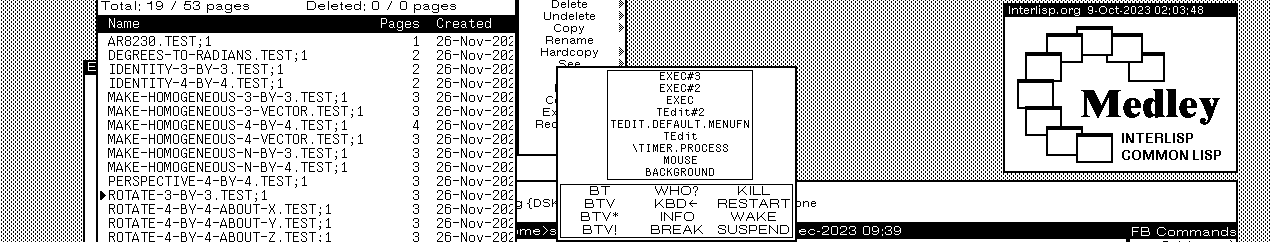
\includegraphics[width=\textwidth]{MedleyShot02t}
  \caption{A screenshot of the current Medley implementation.}
  \Description{A screenshot of the current Medley implementation.}
  \label{fig:teaser}
\end{teaserfigure}


%% \begin{teaserfigure}
%%   \usebox{\verbteaserbox}
%%   \caption{A character-rendered dive into the Mandelbrot set. See Section 6.4 for details.}
%% \end{teaserfigure}

%%
%% This command processes the author and affiliation and title
%% information and builds the first part of the formatted document.
\maketitle

\section{Introduction}
Interlisp.org, a US non-profit organization, is working to resurrect and restore the Medley Interlisp system and has made good progress in modernizing and enhancing it. Medley Interlisp was the last version of the Interlisp system developed by Xerox Palo Alto Research Center (PARC). Accomplishments thus far have included reducing  barriers to entry, making it easier to build versions for modern computing platforms, the creation of an online Medley system accessible through a Web browser, and one-click installers for major operating systems. The Medley software has been released under an open source license, available for download at \url{https://interlisp.org}.

The system's original release came near the end of a fruitful period for interactive software development stretching from the late 1960s through the early 1990s. In the mid-1980s, Xerox PARC tapered off development and moved Medley Interlisp to Xerox AI Systems (a Xerox subsidiary). In the late 1980s, XAIS moved the system to Envos, which closed shortly thereafter and led to a company called Venue acquiring the rights to Medley Interlisp. Circa 2018, Ron Kaplan and Nick Briggs resurrected Medley Interlisp to begin transporting it to modern computing platforms to support natural language research.

In 2020, the Medley Project was formed with the goal of modernizing the Interlisp ecosystem, opening the way for present-day developers to experience its concepts and principles on modern computing platforms like Windows, MacOS and Linux. Interlisp.org was formed to organize these efforts, provide versions of Medley Interlisp to interested users, and provide a repository for source code and documentation. Interlisp.org has been successful in this endeavor as Medley Interlisp now runs on the indicated platforms as well as a browser-based, online version and an ARM version. A Docker container-based release is available for added portability. Interlisp.org has also resurrected several applications including ROOMS, Notecards, LOOPS and others. It has assembled an online Zotero repository collecting Lisp documentation along with Interlisp papers, books, and technical material. Selected source code is also available for contributed programs.

\section{The Project}

Interlisp.org received the source code for Medley Interlisp and its applications from Venue Corporation. Interlisp.org consists of a group of volunteers –- original developers, former users, software historians interested in software preservation, and people interested in software archaeology. This group has focused on:

\begin{itemize}
  \item Modernizing Medley's infrastructure and source code;

  \item Adapting the system to run on modern computing platforms;

  \item Reducing the barrier to entry for new users; 

  \item Resurrecting and restoring Medley Interlisp applications of historical interest; and

  \item Conducting outreach to potential users, students, software historians, and others to provide an understanding of symbolic computing.
\end{itemize}

Notable is Medley's support for two Lisp dialects: Common Lisp and Interlisp. These are implemented as compilers for the respective languages that support REPL-based interaction. While the functions in these languages are implemented in different ways, their data structures are identical, so linked lists, arrays, hash tables and other data types are fully portable between the two languages. This makes it possible to create blended applications in which data is passed between functions written in either language.

%% On the right hand side of the screen are two sets of buttons:

%% Documentation, which open the documentation for standard applications:

%% \begin{enumerate}
%%   \item Provide Basic information from the web site;

%%   \item Provide access to an online Primer describing Interlisp;

%%   \item Access to the PDF version of the 1991 Interlisp Reference Manual;

%%   \item Access to the NoteCards manual; and

%%   \item Access to the ROOMS manual.
%% \end{enumerate}

%% Activate Features, which launch the two applications - NoteCards and ROOMS, which are included in the standard sysout. Other buttons for user-defined applications or system tools and utilities may be added to the opening screen in future versions or by the user.

\section{Adaptation to Modern Platforms}

Interlisp.org is engaged in restoring the Medley Interlisp ecosystem, including tools, utilities, and applications, and provides public versions of source and binary code for modern computing platforms, and available documentation. All of these artifacts are available through Interlisp.org's GitHub and Zotero repositories. The open source version for modern computing platforms consists of:

\begin{itemize}
  \item Maiko, the emulation software that implements the Interlisp Virtual Machine;

  \item Medley, the source and compiled versions of Medley Interlisp, its tools and utilities, and selected applications; 

  \item Installers for modern computing platforms – Windows 10+, MacOS, Linux, including WSL, Raspberry Pi; and

  \item \url{online.interlisp.org}, a browser-accessible on-line version of Medley Interlisp.
\end{itemize}

Additionally, Interlisp.org provides public access to its Zotero repository, which contains a collection of documentation for Interlisp and other Lisp implementations.

\section{Reducing Barriers to Entry}

Easy access to Medley Interlisp will help (re)introduce potential users to Interlisp in a way that allows them to learn and experience its features while building their expertise. Interlisp was developed before current conventions for mouse and window-driven software development as well as Unicode's standards for textual representation. Medley has been modernized to give the users the look and feel that they are accustomed to current systems.

%% ===

Interlisp.org created an online version of Medley Interlisp using Docker and Amazon Web Services, providing for users to experience the system through a web browser without running any of the Medley system's components on their local computing platform. When they are ready, if they choose, they can install a version of Medley Interlisp onto a local computer system and download files created through the online version to be used on the same system.

Online Interlisp has 428 registered users who accounted for 1685 online sessions during 2023. In addition, there were 2,588 anonymous guest user sessions.

\section{A Model of Interactive Software Development}

Medley Interlisp was created to provide a computing environment for research into and development of large-scale applications. To this end, Xerox PARC users as well as others developed tools and utilities to facilitate software development in an interactive, graphical user interface (GUI) in a collaborative environment.\cite{Kaisler2021} Among these tools and utilities were MasterScope, Spy, DWIM, CLISP, and LOOPS. Some of these tools and utilities have yet to appear in modern software engineering systems. Over 100 tools and utilities are represented in the LispUsers library of contributed software.

Numerous tools were developed at other institutions than Xerox PARC, such as NASA, several DARPA contractors, and private commercial firms. We are searching to identify these tools and utilities; acquire, where possible, source code; modernize them to run on modern computing platforms; and make them available, with appropriate licenses and permissions through the GitHub and Zotero repositories.

%% bug reported by paolo - sharpsign, paren, sharpsign - error - 

\section{Interlisp in Perspective}

The history of Interlisp parallels the history of the early years of artificial intelligence research as many AI researchers had access to DEC PDP-10/DEC System-10 computer systems which could run relatively large programs in an environment\cite{Bobrow74} with 256K words of real memory. Interlisp provided a residential programming environment in which the standard software development functions of edit, compile, link, and execute, along with preparation of documentation, could be conducted without leaving the Interlisp environment\cite{Teitelman73}.

In Interlisp, a user edits and evaluates Lisp objects that reside in an in-memory image. The code is saved to files that are more like code databases than traditional source files. Users do not edit the files, but load file contents into memory to edit, compile, and execute. Medley Interlisp keeps track of the changes that the user makes to source code that have been made by using the SEdit structure editor to edit in-memory objects. The File Manager provides a simple interface that archived the changes to the code to disk when the user closed a session or invoked a function. The beginning of a file specified metadata, which described the ``file environment'' and readtable associated with the file.

The File Manager coordinates the development tools and readable code management tasks. It notices the changes to Lisp objects edited with SEdit or manipulated in memory, tracks what changed functions and objects need to be saved to symbolic files, and carries out the actions for building programs such as compiling or listing them (like some of the functions of Unix make).

This model is unique even today as no programming system apart from Smalltalk provides the same capabilities. As Smalltalk was developed concurrently with Interlisp, many of the ideas percolated between the development groups at PARC, albeit with different implementations.

Although Interlisp was not the first version of Lisp (there were several on mainframes and early minicomputers), it is safe to say that it influenced most succeeding versions. While Interlisp was implemented on top of a virtual machine, preserving vertical integration, and many applications were written in Interlisp, most other Lisp systems were written in an imperative programming language, such as C, for performance reasons.

\section{Medley Interlisp Ecosystem}

The Medley Interlisp Ecosystem includes the following components:

\begin{itemize}
  \item Maiko, the emulator software for the Interlisp virtual machine;
  \item Medley Interlisp, the Interlisp source code and its utilities and tools;
  \item Applications, including several Interlisp applications, such as ROOMS, Notecards, LFG, STRADS, IDA, as well as other Lisp system applications; and
  \item Documentation, a comprehensive collection of books, papers, technical memoranda, and manuals regarding Interlisp, and extending to other Lisp variants.
\end{itemize}

Interlisp.org welcomes contributions of source code and documentation to add to its repositories.

The following sections briefly describe each of these components and the work done to make them operational. The descriptions hereafter can only faintly reflect the effort expended by many people to restore, modernize, and document Interlisp software.

\subsection{Maiko}

Maiko is the emulator that implements the virtual machine upon which Interlisp runs.\footnote{\url{https://github.com/Interlisp/maiko}} Maiko was initially developed by Fuji Xerox but acquired by Xerox PARC, which continued to maintain and enhance it. Written in Kernighan and Ritchie C, Interlisp.org developers have modernized it, making it ANSI C compatible. A few of these modifications included resolving issues of signed vs. unsigned characters, adding prototypes for functions, ensuring all parameters have types, fixing some errors in incorrect translation of Lisp code to C code, and optimizing all virtual machines' opcodes. 

This modernization facilitated the transport of the Medley Interlisp ecosystem to modern computing platforms with some effort. Numerous programming changes were made to ensure that Maiko could run on Windows 10/11, MacOS versions, and Linux and WSL-based platforms, as well as an online version accessible through browsers that runs within a Docker container.
 
\subsubsection{Running Natively on Windows 10/11}

Previously, running on Windows required the use of the Medley Docker container or WSL. Both required significant effort to set up along with knowledge not possessed by most Windows users. Native support was developed using Cygwin and SDL2, allowing the development of a one-click installer in the form of an \texttt{.exe} file.

\subsubsection{Support for AArch64}

The build scripts for the Maiko virtual machine were extended to support the AArch64 (ARM) platform under the Raspberry Pi Bookworm and later. This effort established the model for future extensions to generate build scripts for other platforms. Any system which has an ANSI C compiler can host a version of Medley Interlisp.

%% \subsubsection{Build and Release Automation}

%% Within GitHub, the build and release process for all major components was automated, including Maiko, Medley, Notecards, and the online system. The build, loadup, and release tasks run weekly which has improved our ability to integrate and deploy fixes and enhancements to these systems on a weekly basis.


\subsubsection{Major Platform Installers}

Installing Medley was a multi-step process, which required some expertise with the administrative tools of each major platform. A ``single-step'' installer using a ``one-click'' approach was developed for MacOS, windows (native), Windows running WSL and Cygwin, and many Linux distributions, which allows a Medley user to quickly and easily install a Medley release and begin exploring or performing effective work.

\subsection{Medley Interlisp}

Medley Interlisp comprises the basic code implementing the Interlisp language and environment as well as a considerable selection of tools and utilities. Because the tools and utilities were written in Interlisp, many of these run without major changes once the basic system became operational.

\subsubsection{Common Lisp Support}

With the groundswell of support for Common Lisp in the mid-1980s, Xerox PARC extended the Interlisp environment to support Common Lisp, specifically, as of Common Lisp: The Language, Version 1 (CLtL1), along with CLOS and CL's condition system. The infrastructure supporting Interlisp and Common Lisp is completely integrated such that selection of functionality by either Interlisp or Common Lisp depends merely on the use of packages.

%% ^^ WHAT DOES THIS MEAN?

%% For example, two versions of the Exec window are initialized as shown in Figure 1 – one using the Interlisp Readtable and functionality selected by the package IL: and one using the Common Lisp Readtable and functionality selected by the package CL:. Both can be used in the same application with transition between the two variants, but there are some rough edges we are working out.

The Common Lisp integration with the Interlisp tools was incomplete. Substantial work has made it easier to use many of the Interlisp tools and utilities, such as HELPSYS, DWIM, and MasterScope. Also, some of the functions and directives in CLtL2 are not available (such as 'declaim' versus 'proclaim'). As we discover these we are determining how to provide the missing functionality, but some might not be available until later in 2024.

\subsubsection{Editing and Browsing Support}

Since the early 1980s, Medley Interlisp has had a 16-bit internal representation of characters in strings and atoms using the internal Xerox XCCS codes\cite{Nuyens86}. These codes have been mapped into the appropriate glyphs for display and printing. The character reading/writing functions have been generalized in the external format project. If a file's external format is specified as UTF-8 when a stream is opened, UTF-8 byte sequences are read into 16-bit (Unicode) codes, which are translated into their XCCS equivalents before being delivered to the calling function. Support for ISO8859 and certain Japanese conventions are also provided. These external formats push the coding and format concerns to the periphery of reading/writing, thus isolating the internal processing functions\cite{Kaplan21}.

TEdit, the text editor, was extended with UTF-8 support that improved system efficiency, reliability, and maintainability\cite{Xerox86}. TEdit reads all characters into an internal editing buffer and creates pointers to the bytes on the file that represent those characters. It only interprets those bytes when it needs to display that section of the file, move characters from one place to another in the file, or copy them to some other application. Thus a TEdit session on a large file opens quickly and only occupies a small amount of memory.

TEdit has consumed a major portion of the modernization effort over the past three years because assumptions about the XCCS file format were threaded all through the core TEdit implementation. Every location of XCCS code usage had to be tracked down. This revealed a variety of bugs, glitches, inconsistent behaviors and maintainability issues, which required substantial refactoring. As of Spring 2024, this effort is finally coming to the end which has significantly improved the robustness and reliability of the Medley Interlisp system.

Additional changes allowed the ingestion of Xerox Alto Bravo-format files, making it possible for legacy documents to be converted to PDF through invocation of an external converter. Also, HELPSYS was extended to allow lookup and display of the Common Lisp Hyperspec and other Medley documentation.

\subsubsection{PDFStream}
Medley incorporated a native imagestream implementation for producing PostScript™ hardcopy files. The PDF format is not supported as it was not yet invented when this system was developed, but an interim PDF solution from 2023 allows creating a PS file and executing a UnixUtils shell script to convert it to PDF via Ghostscript's ps2pdf utility. Medley's FileBrowser was extended to automatically open PDF files in a separate window using a host-resident PDF viewer.

\subsubsection{UnixUtils}

Medley was enhanced to allow it to reach out to the host environment platform to accomplish system-level tasks that are not available in Medley. These included ShellBrowser which opens a URL in the specified browser, and ShellOpen which opens a host-resident PDF viewer on the specified file.

\subsubsection{Github Integration}

Github is being used to manage the coordination of multiple developers across several time zones and countries in extending Maiko, Medley, and the tools and utilities. A major effort was the integration of Github functions with the Interlisp File Manager. GitFnS is a set of functions that include a menu-driven interface to compare Lisp source files on a function-by-function basis that supports the ``residential style'' development tools of Interlisp.

\subsubsection{Mouse and Keyboard Usage}

Originally, Interlisp supported the three-button mouse available on the Xerox custom processors. These seem to have largely disappeared, so major effort has focused on making it work with two-button (such as Windows), one-button (such as Macs), or use of a touchpad cursor. Function keys on several popular keyboards have been mapped to codes for other mice varieties to allow access to the functionality. A ``meta'' key allows emulation of the middle mouse button of the three-button mouse. Implementing some scroll wheel and middle mouse button functionality is still a work in progress.

Originally, there were just a few keyboards available when Interlisp was developed. Every application did its own decoding of keys to map then to internal codes. This is impossible now. Users want uniform treatment, no matter which keyboard they use. Interlisp.org is working hard to develop mastery over keyboard encoding and communication because keyboard handling is buried in several different locations within Maiko and Medley. Some tools and utilities also interpret keys differently.

Our goal is to have a unified keyboard model that will accommodate a large number of commercial keyboards. This is likely to involve some translators for keyboards or translators to some internal model for key handling. Work has begun by the Interlisp.org team to develop a set of keyboard mappings prior to developing a single keyboard model that would unify keyboard handling of tools, utilities, and applications. We expect this will improve the efficiency of setting up a new environment on a different computing platform.

\subsection{Applications}

Numerous applications have been built using versions of Interlisp including many early AI tools as well as ROOMS\cite{Henderson86}, NoteCards\cite{Xerox85}, a workbench for writing LFG grammars\cite{Kaplan03}, Intelligent Database Assistant (IDA), LOOPS, and the Strategic Automated Discovery System (STRADS). Recently, an affiliate of Interlisp.org discovered an archive of the Stanford AI Laboratory, which contained several programs, including sources for Doug Lenat's AM and Eurisko programs\footnote{\url{https://white-flame.com/am-eurisko.html}}. These were written in an early version of Interlisp. Interlisp.org has demonstrated they can be loaded into a Medley Interlisp environment with minimal changes and are documenting how to make them usable again.

Interlisp.org is collecting open source Common Lisp programs and using them to test the Common Lisp implementation, making some changes to make them easier to use, and making them available through our GitHub repository for public use. Some of these applications include ATMS, BB1, NIKL, and several Common Lisp programs. Work will continue throughout this year to get them running in Medley reliably and provide minimal documentation (or more, if available).

\subsection{LOOPS}

The Lisp Object-Oriented Programming System (LOOPS) is unique in programming systems in that it incorporates four programming paradigms:

\begin{itemize}
  \item Imperative/Functional Programming
  \item Object-Oriented Programming
  \item Aspect-Oriented Programming
  \item Rule-Based Programming
\end{itemize}
    
The integration of these paradigms provided the software architect and developer with a comprehensive, powerful programming environment for building complex applications\cite{Bobrow83}. The Medley Interlisp tools and utilities were extended to operate with the LOOPS constructs seamlessly. The integration of these paradigms in a single system allows the software architect/programmer to choose a representation of data and problem solving capability that best meets the needs of the application. The graphical user environment supported by the Medley Interlisp environment allows the creation of gauges that can provide interactive displays of the values of variables to which they are attached.

Researchers at PARC developed the Truckin' game to help users understand how to program in a multiparadigm environment and to visualize what was happening as the game evolved\cite{Stefik83}.

LOOPS is documented in three books that address the Basic System, the Tools and Utilities, and the Rule-Based System. The latter volume introduces the Truckin' game\cite{Stefik00}, which was developed by researchers at Xerox PARC to teach users how to develop complex applications in LOOPS. We anticipate showing how to create an Adventure-type game in LOOPS as an element of the book.

%% ADD: Knowledge-based system info like from Friedland?
%% ADD: Medical system like INTERNIST from Myers?

\subsection{Documentation}

Interlisp.org has access to a wide variety of documentation about Interlisp and Common Lisp, including original Xerox PARC memoranda, manuals, and program and application documentation in the computer History Museum's PARC archive. Much of this documentation was written by the original developers who already knew how to use the system, but is obtuse for new users trying to understand how to use it. Interlisp.org has developed additional volumes for how to use Medley Interlisp and LOOPS since 2021, all of which are available at Interlisp.org. These include:

\begin{itemize}
    \item Interlisp: The Language and its Usage
    \item Medley Interlisp: The Interactive Programming Environment
    \item Medley Interlisp: Tools and Utilities
    \item LOOPS Volume I: The Basic System (Draft available at Interlisp.org)
    \item LOOPS Volume II Tools \& Utilities (Draft available at Interlisp.
    \item LOOPS Volume III: Rule-Based Systems (In progress, forthcoming)
\end{itemize}
    
Additional work is planned for the other applications and for Common Lisp and its applications over the next two years. This documentation is focused on new users of these applications. 

\subsubsection{Community Outreach}

Interlisp.org revamped its website over the past year to make it easier for prospective and experienced users to navigate and support further Medley Interlisp development. The website provides access to most of the material that Interlisp.org has collected. Additional information is continually being added as we find new sources. Information search and retrieval was extended beyond the website to the GitHub repository and the Zotero repository.

%% Numerous link errors and 404 errors were corrected. 

%% Interlisp.org worked with Eric Kaltman from the University of California Channel Islands  and some of his students to help organize files in the  repository. He has moved to the University of Alberta, Calgary, Alberta, Canada and will continue his interaction with us.

Interlisp.org continues its technical outreach to the broader Lisp and Computer Science community through technical presentations. Three talks were presented this past year:
\begin{itemize}
    \item BALISP: In March 2023, the project's efforts were presented to the Bay Area Lisp meetup group. The slides are available on the project's Google Drive\footnote{https://drive.google.com/file/d/1xpXSoEnc5PPnIa7BHcionBbc8v-Nxp7N/view?usp=sharing} and the talk was on Youtube\footnote{https://www.youtube.com/watch?v=N1MobfEaoWY}.
    \item Software Preservation Network (SPN): On November 2, Larry Masinter presented to the SPN Idea's Workshop technical details of our work as well as suggesting future collaborative projects across the community.
    \item BCS Computer Conservation Society (CCS): Steve Kaisler presented a talk entitled ``Software Archaeology: The Medley Restoration Project'' to the CCS Monthly Meeting on November 16 in London, England. It included a brief history of Interlisp, a brief review of some applications, and some issues and challenges in in modernizing Medley Interlisp (some of which have been presented in this paper).
\end{itemize}

Articles regarding Interlisp.org and the Medley Interlisp Project have appeared in Hackaday, Hacker News and The Register\cite{Proven23}.

\section*{Acknowledgments}

We acknowledge the leadership and historical perspective of some of the original developers - Larry Masinter, Nick Z. Briggs, Frank Halasz, Ron Kaplan and the other members of Interlisp.org. We also acknowledge the estate of John Sybalsky for granting the rights to use and distribute the source code for Medley Interlisp. And, to Eric Kaltman and his students at UC Channel Islands for efforts in organizing the Zotero repository. Funding for this effort has been provided members of Interlisp.org.

%%
%% The next two lines define the bibliography style to be used, and
%% the bibliography file.
\bibliographystyle{ACM-Reference-Format}
\bibliography{ILPaper}

\end{document}
\endinput
